\title{Master of Science \\ Organizational Management (Human Services) \\ Graduate Portfolio}
\author{Dustin Kindred \\ Chadron State College}
\date{\today}

\documentclass[12pt,titlepage]{article}
\usepackage[final]{pdfpages}
\usepackage[letterpaper, margin=1in]{geometry}
% todo: Make Active navigation Links in Table of Contents
\begin{document}
\maketitle
\tableofcontents

\section{Part I}

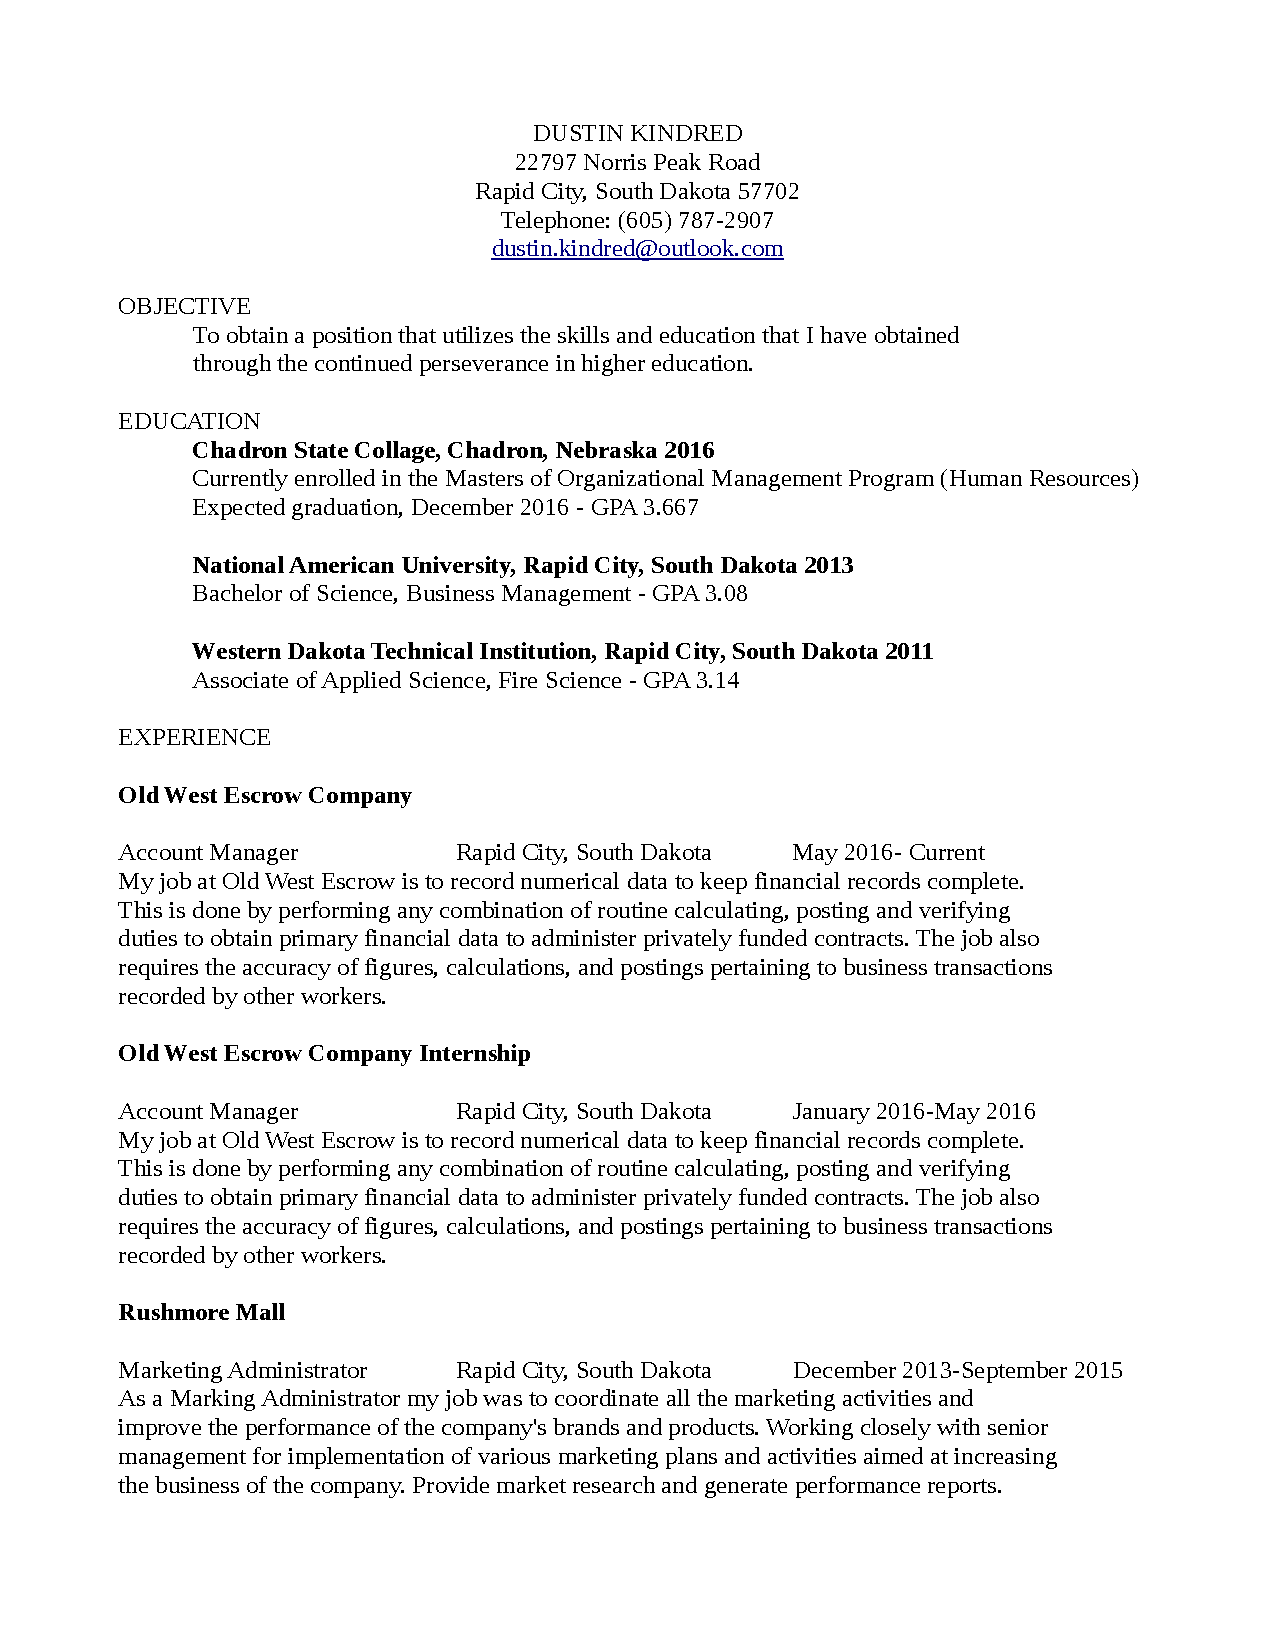
\includepdf[pages=1,pagecommand={\subsection{Resume}}]{resume.pdf}
\includepdf[pages=2-]{resume.pdf}
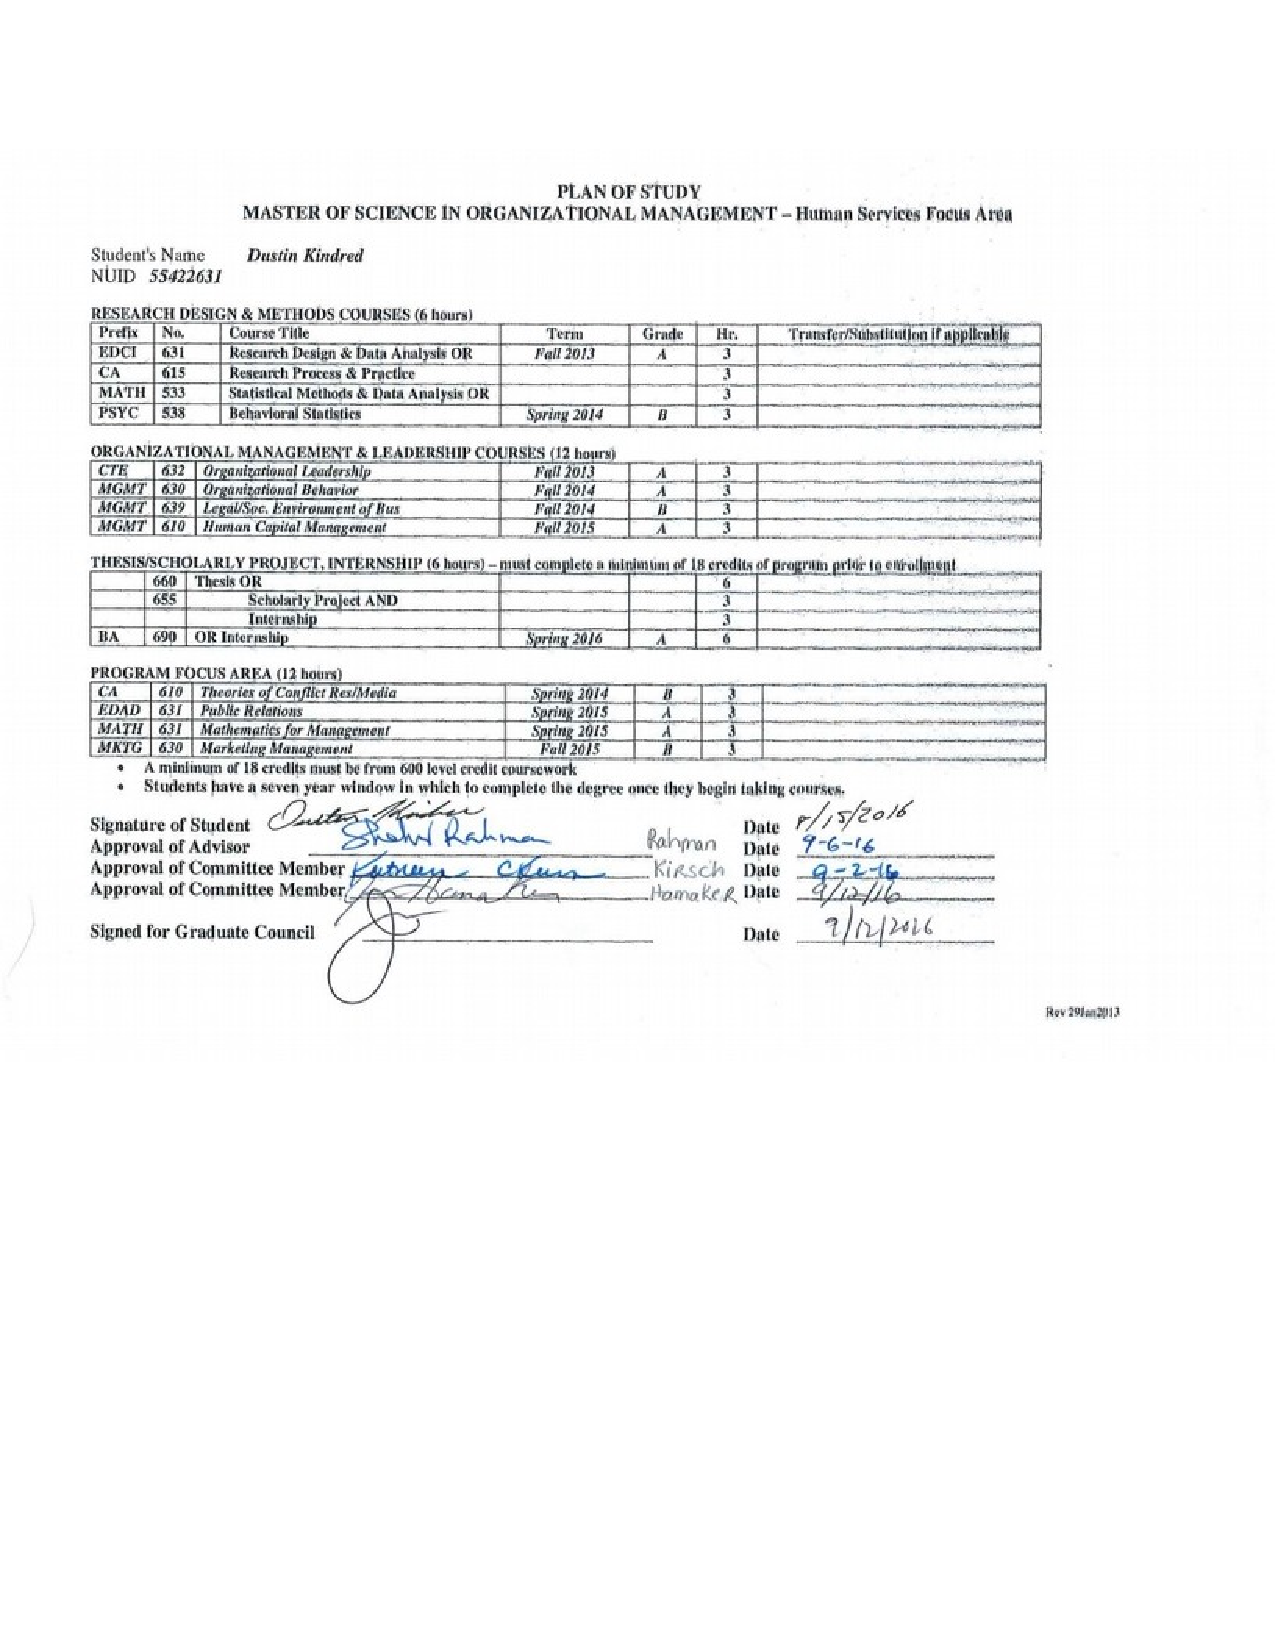
\includepdf[pages=1,pagecommand={\subsection{Plan of Study}}]{planofstudy.pdf}

% Part 2
\section{Part II}
% Part 2 Research Design
\subsection{Research Design and Data Analysis}
\subsubsection{Reflections}
\paragraph {}
Research and design analysis was an interesting class. The class was also my most feared class that could have taken. I am not a prolific writer by any means. My writing currently lacks style and the flare that I have come to expect when reading academic papers. However, this class helped a great deal in regards to feeling comfortable with my writing style. The areas in writing that I lacked then are still my faults on my writing today I am just getting better at spotting the errors. This was not the only purpose of the class. The purpose was to understand the basic research and design process to better understand the methodologies used in academic research. The course met this purpose and exceeded expectations. Dr. Blundell was excellent with the delivery of her instruction and returned assignments with helpful notes to the student showing where we could perform better and expand on our ideas.
\paragraph {}
The current course objectives were to comprehend research design and statistical analysis while applying common descriptive comparative and predictive procedures to selected data. The last objective was to create an original research problem and develop an integrated literature review and propose related research from this plan. All objectives I felt were met throughout the course. The course was a nice break-in course for advanced behavioral statistics giving a nice introduction to the class that was taken at a later time. Because we went through the fundamentals of statistical data and what it means as we read other academic reports I was able to infer whether I needed more material to back my claims as we went through an original research problem.
\paragraph {}
For the original problem I chose to focus in an area that I was currently working. I was working in emergency mental health confronted with an organizational goal of reducing arrests among the mentally ill community. Here I struggled a bit at refining my research problem into quantifiable terms. At first the problem was too vague and gave little to a researchable answer. Dr. Blundell was excellent at providing direction in this regard. After refinement I choose to narrow the topic to the use of intervention teams in conjunction with psychiatric emergency services. After performing the literature review process and writing the final paper I was confident to say that the issue still needs more research to solve the specific topic. While working in the capacity of my position I would have loved to be able to actually perform the specific study and feel that this class enable me to exude the confidence needed to go forward with the study if I had the chance.% Fall 2013
% Syllabus
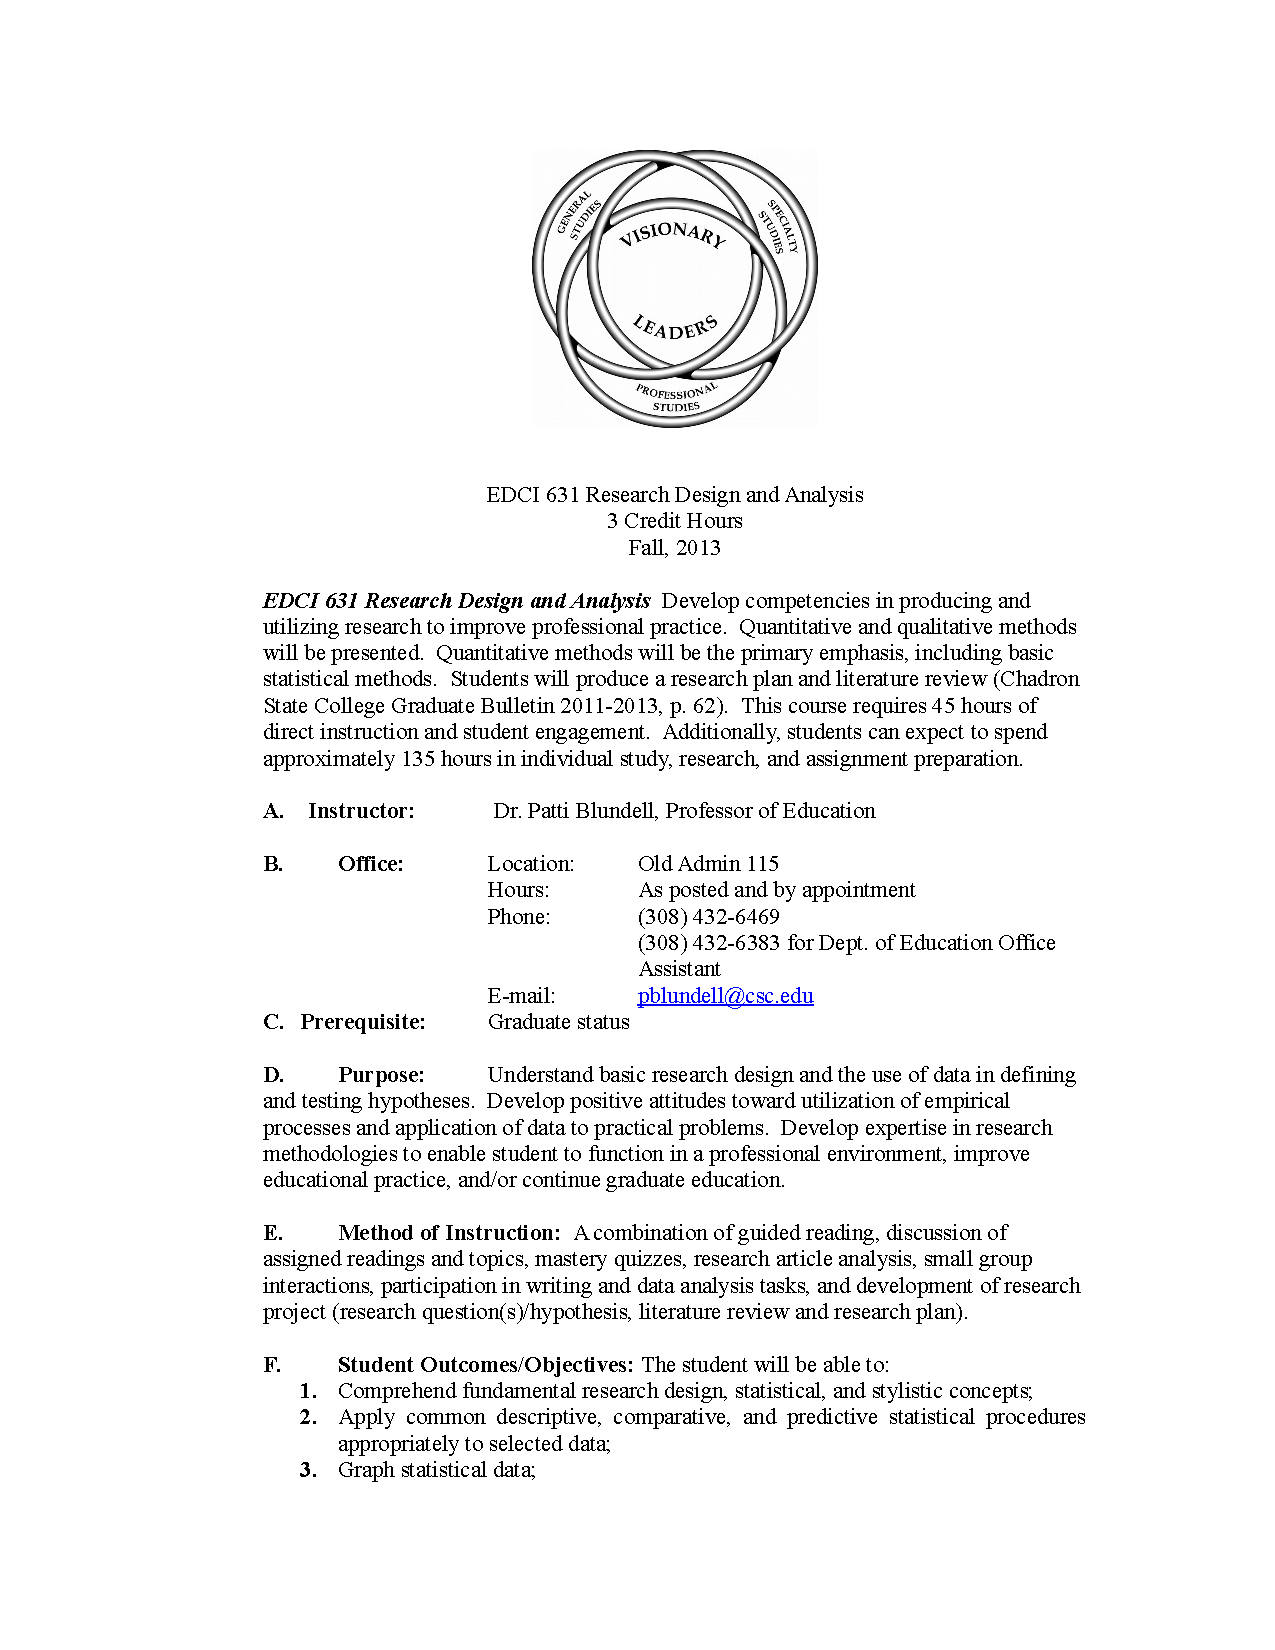
\includepdf[pages=1,pagecommand={\subsubsection{Research Design and Data Analysis Syllabus}}]{EDCI631syllabusfall13.pdf}
\includepdf[pages=2-]{EDCI631syllabusfall13.pdf}

% Work Examples

\includepdf[pages=1,pagecommand={\subsubsection{Work Examples}}]{Reducing_Arrests_&_Hospitalization_working_draft.pdf}

\includepdf[pages=2-]{Reducing_Arrests_&_Hospitalization_working_draft.pdf}

% Part 2 Org Leadership
\subsection{Organizational Leadership}
\subsubsection{Reflections}
% Start of Reflections
\paragraph {}
Organizational Leadership or CTE 632 was easily one of my favorite classes that I had taken and was looking forward to participating in. I felt that this class was one of the premier cornerstone classes to the degree program. I was happy that the class didn't have a required textbook rather we used a variety of different readings that Dr. Nealeigh had provided to us as we went through the different leadership styles. I found this teaching methodology more interesting and engaging than using a textbook. I also really like the book project where we had read a book on an inspirational leader and compare them to leadership styles found in other books. This helped the class feel engaging through applied critical thinking.
\paragraph {}
I learned that there are 6 leadership styles that are commonly practiced. Even though we have these six styles we may fall into the trap of conforming to just one style and make the best of it. However, this is not advantageous to us as leaders. As leaders we need to recognize the situation and then apply the correct style to the situation. A great example would assume that I fall into the democratic style of leadership. This is a great style and forces everyone to work and contribute together. This style ,however, is not beneficial in emergency situations. In these scenarios the leader needs to make quick direct decisions based on the rapidly evolving conditions. In this situation I would need to switch gears and become a coercive leader. As future leaders we cannot convince ourselves that there is only one style of leadership that is the best for everyone. We need to become fluid and adapt as needed.
\paragraph {}
During the course we also learned about organizations and how they are setup with a vertical leadership structure for horizontal structure. Organizations can also be compartmentalized or non-compartmentalized. Again, these hierarchies are based on what works for the organization and does not work for every situation. I have found that in smaller organizations it will make more sense to deploy the horizontal or flat structures.
\paragraph {}
Perhaps the best part of the class was reinforcing the concepts of power and empowerment as it relates to employees and how employees react to these methods. I particularly take to the concepts of employee empowerment as it relates to job function. As leaders we need to recognize employees that are able to expand beyond their designed job functions to encourage growth and job satisfaction. We also need to understand that job enlargement can also add undue stress in the workplace when we enlarge too much. In situations such as this we need to consider if the employee needs to take on a new job title to recognize the work they are doing for the organization or if we need to hire other employees to reduce the workload balance conundrum. In either situation this class has giving tools that will be used everyday. The theories and concepts may not always be on the forefront of the mind daily, but are well instilled in my leadership style. Currently my leadership style is a mixture of authoritative and democratic. % Start Syllabus
\newgeometry{top=.3in}
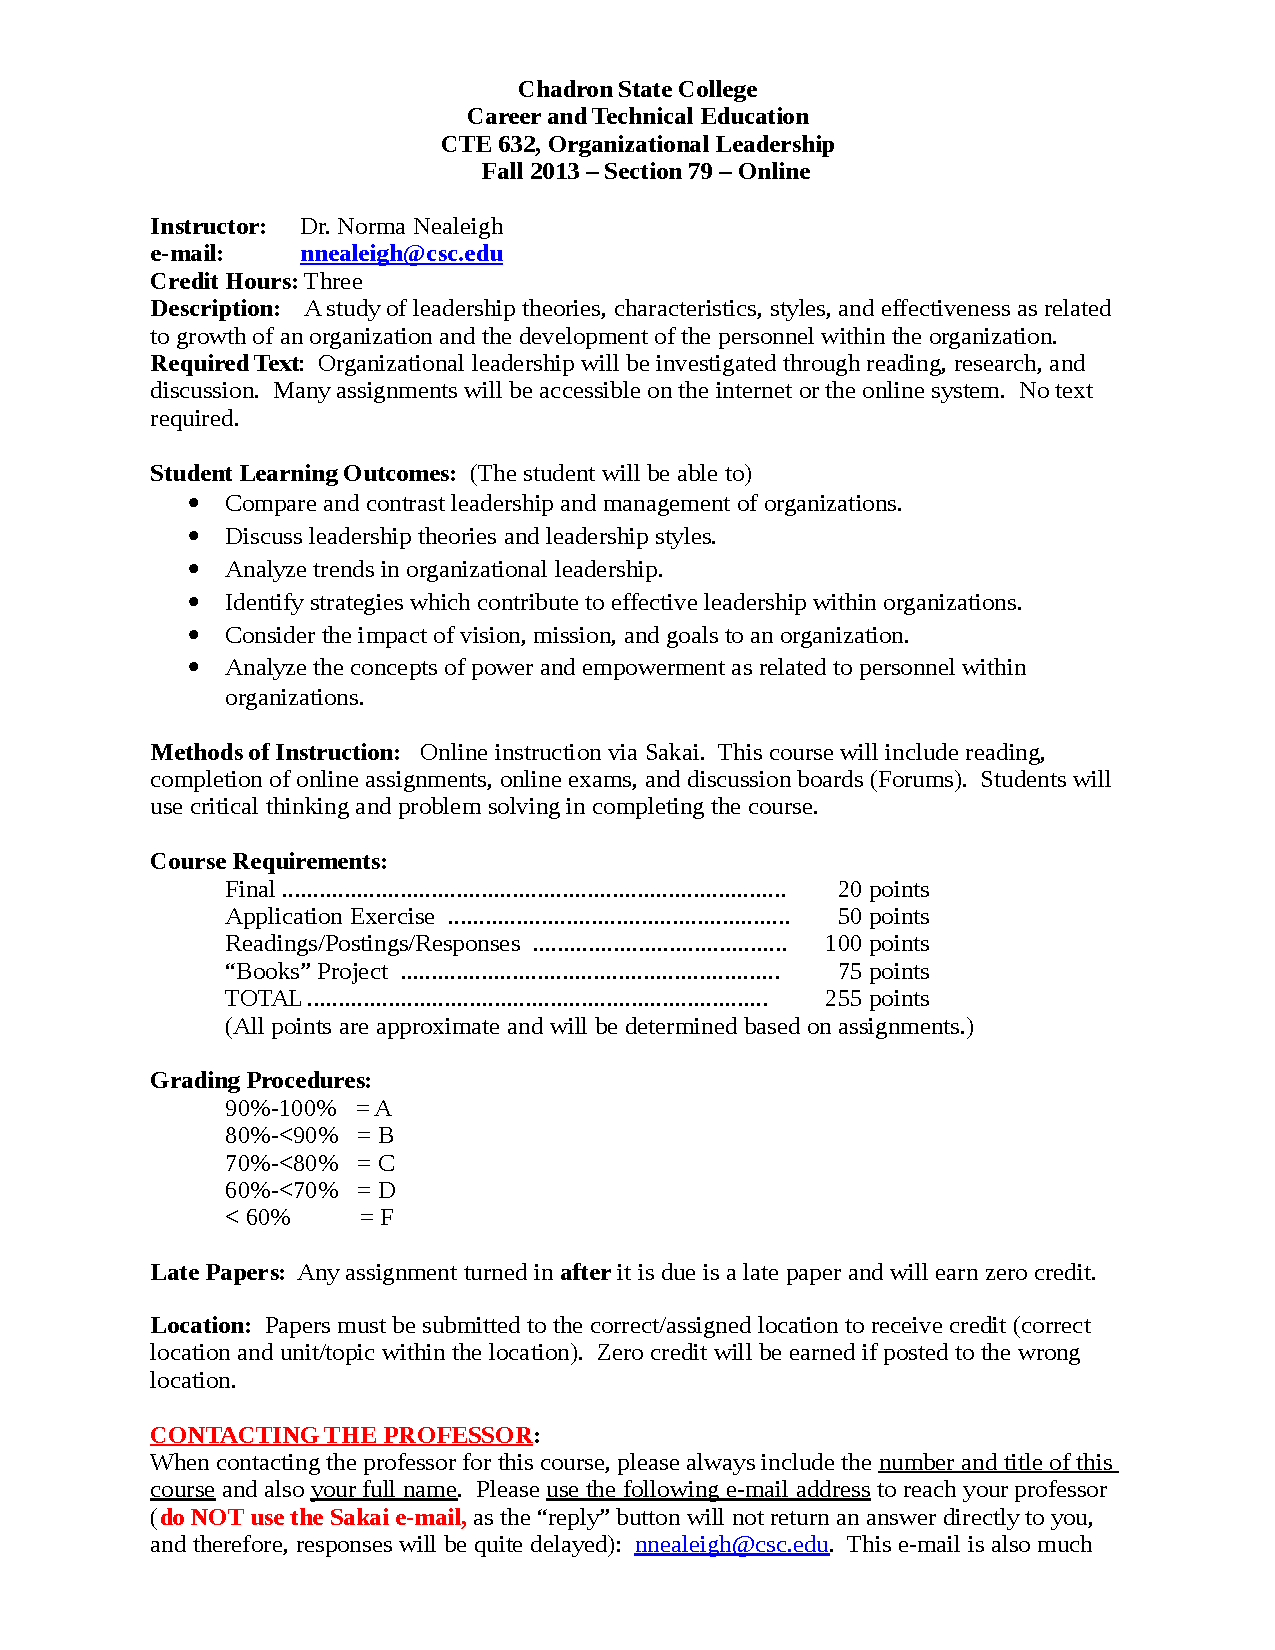
\includepdf[pages=1,pagecommand={\subsubsection{Organizational Leadership Syllabus}}]{CTE632SylbsOnLine139.pdf}
\restoregeometry
\includepdf[pages=2-]{CTE632SylbsOnLine139.pdf}

% Work Examples
\newgeometry{top=.3in}
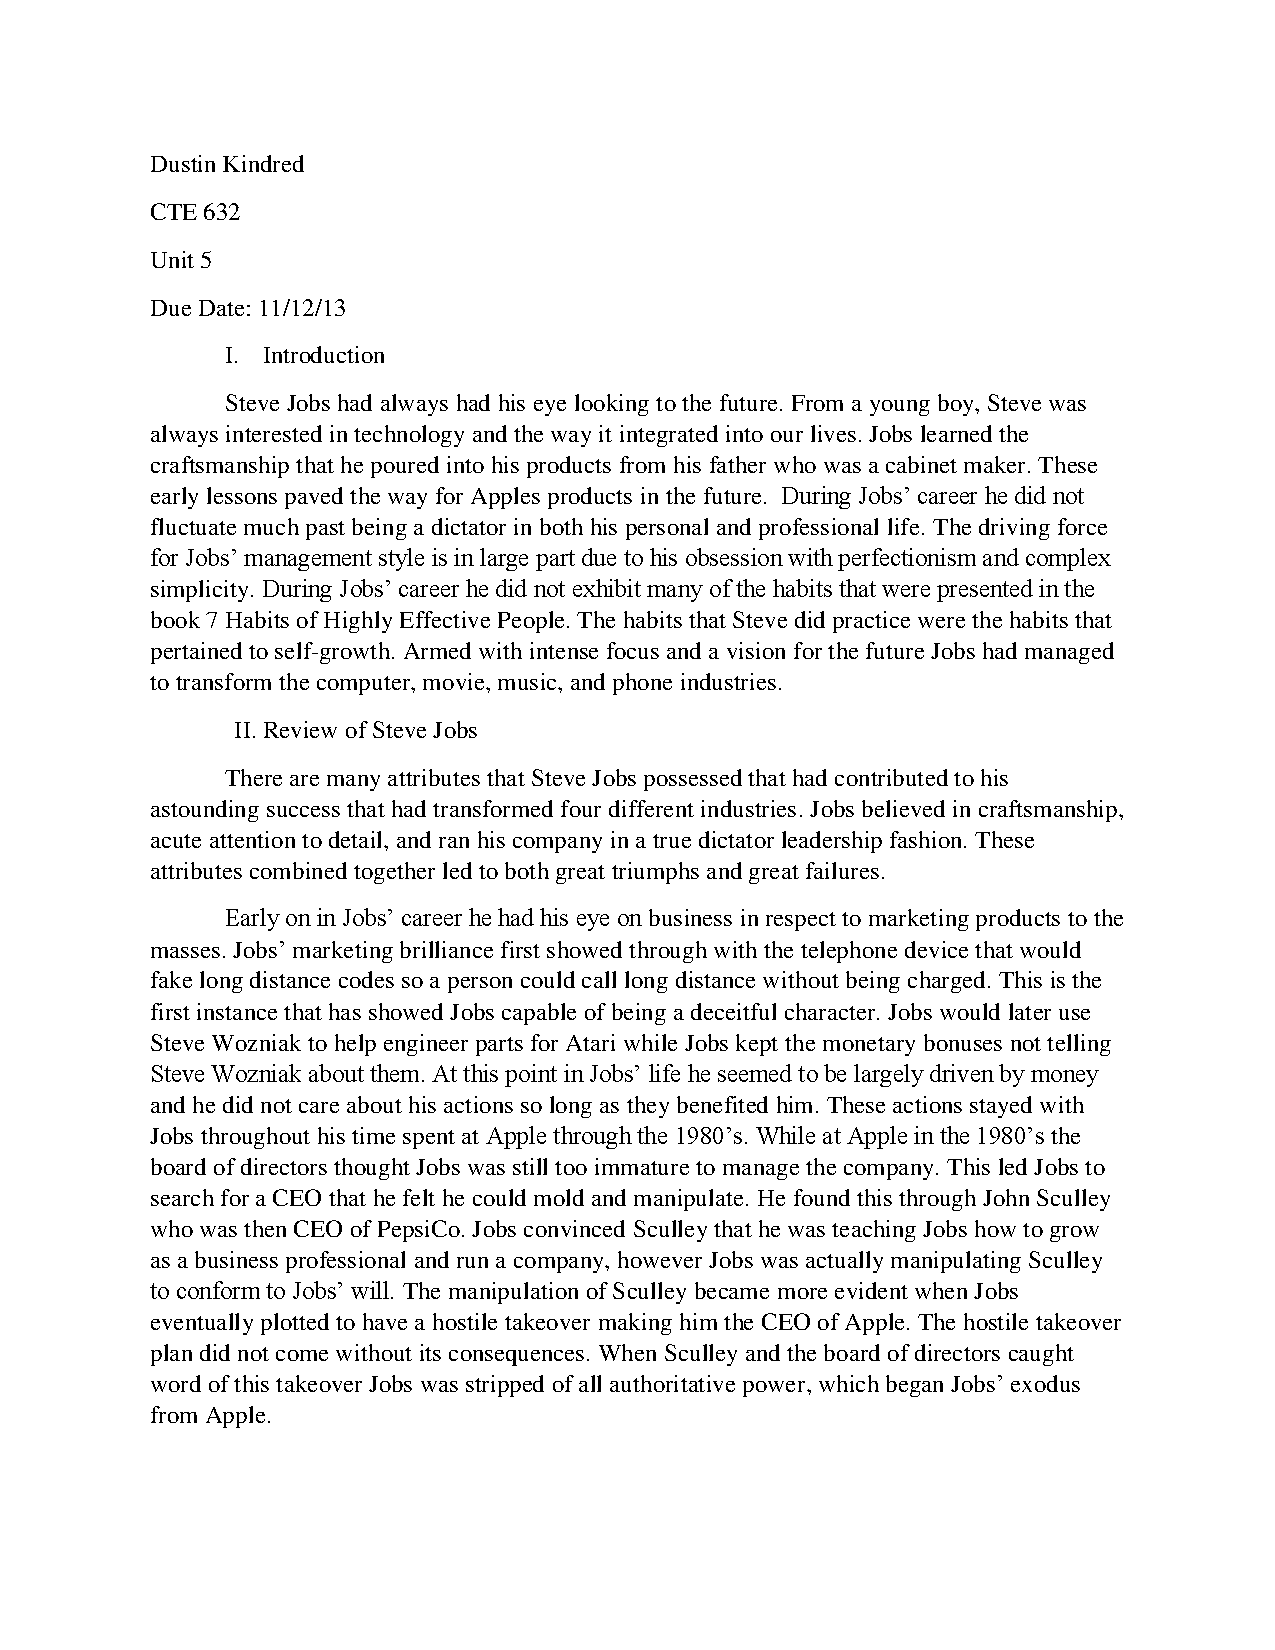
\includepdf[pages=1,pagecommand={\subsubsection{Work Examples}}]{Book_review.pdf}
\restoregeometry
\includepdf[pages=2-]{Book_review.pdf}

% Spring 2014
\subsection{Advanced Behavioral Statistics}
\subsubsection{Reflections}
\paragraph {}
This class used a online format of teaching where are assignments were designed by software including online textbook. I find this format very difficult to interact with and felt that much of the learning was more self learning and not learning from the instructor. Many times when figuring out assignments I would need to seek out other resources to understand the concepts in order to do the homework. This is not the sole fault of the professors teaching, but rather an issue with course work that relies on online software based math courses. Since the course was laid out with software learning this lead to just solving problems without hitting on the course learning outcomes.
\paragraph {}
Throughout the class I did become more familiar with performing ANOVA and CHI Squared tests. Since this course picked-up where my introduction to statistics course left off and I was happy to finish learning some of the more advanced statistical methods. But I did have a hard time grasping the concepts presented in the class and was left wanting more direction in each lesson than the course software provided.
\paragraph {}
What I have taken away from the class is even though I could not recite how to perform some tests today. I do know what types of tests I should be performing in order to arrive at a statistical result. If presented today to perform a statistical analyses I would need to refresh my memory of what is needed in order to give an exact result. I don't feel this is a bad outcome because I am not ignorant to the statistical process.
\newgeometry{top=.3in}
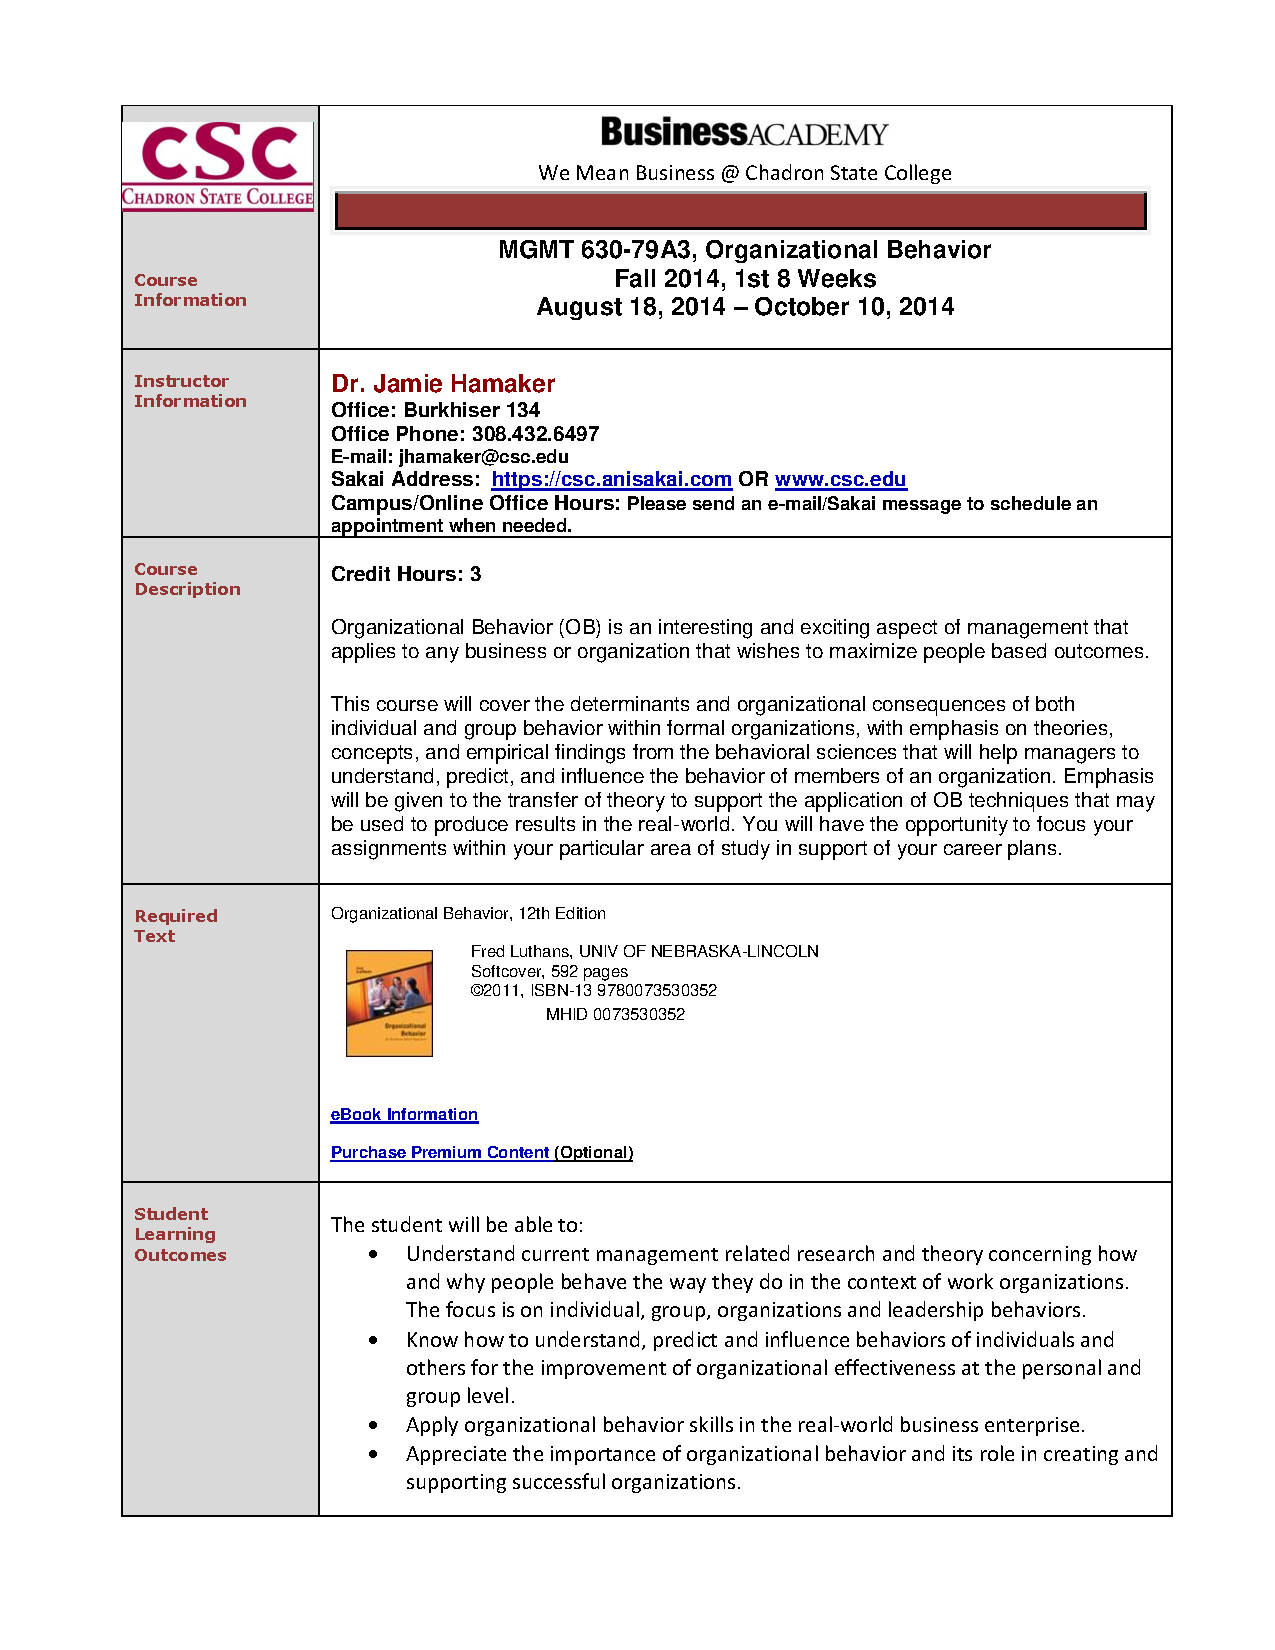
\includepdf[pages=1, pagecommand={\subsection{Advanced Behavioral Stats}}]{Syllabus_MGMT630.pdf}
\restoregeometry
\includepdf[pages=2-]{Syllabus_MGMT630.pdf}

\subsection{Theories of Conflict Resolution}
\subsubsection{Reflections}
\paragraph {}
Conflict Mediation was a hard class for me. Although I use the underlining concepts of this class everyday at work when working with customers. From the moment we started I was wishing the workload would have been lighter. I say this because I felt that the discussion response requirements were so much that the class created an atmosphere of forced response. I understood the purpose of the original in depth discussion. I also understand the purpose of responding to other participants. What I did not understand was the purpose of responding to three other posts with the same in depth response that was required with the original post. I really struggled in writing the in depth responses to three other students and felt that my responses were not genuine and forced as I struggled to meet the requirements of the class. Many times most of the students had close to the same response to the original post which lead to the question of how am I going to write 14 paragraphs three different times explaining how we have a similar experience and perspective. I would have liked to see the requirement for responses limited to “food for thought, insights gained and lessons learned.”
\paragraph {}
From taking this class I have learned that to every decision and every outlook there is a cause for the conflict. Everyone has their own personal perspective and perceives the world differently than the other. Because of varying perspectives we have to work hard to see the world from the other point of view. Once we accomplish this we can work together to create a common ground in which we can work from. The main take away from the class is we all need to take a moment to listen to other and to not speak out of emotion. This is what I understood from the S-TLC system. We must stop then think about what we are listening to then communicate. This acronym can be used just about every conflict from interpersonal to work/co-worker related conflicts.

\newgeometry{top=.3in}
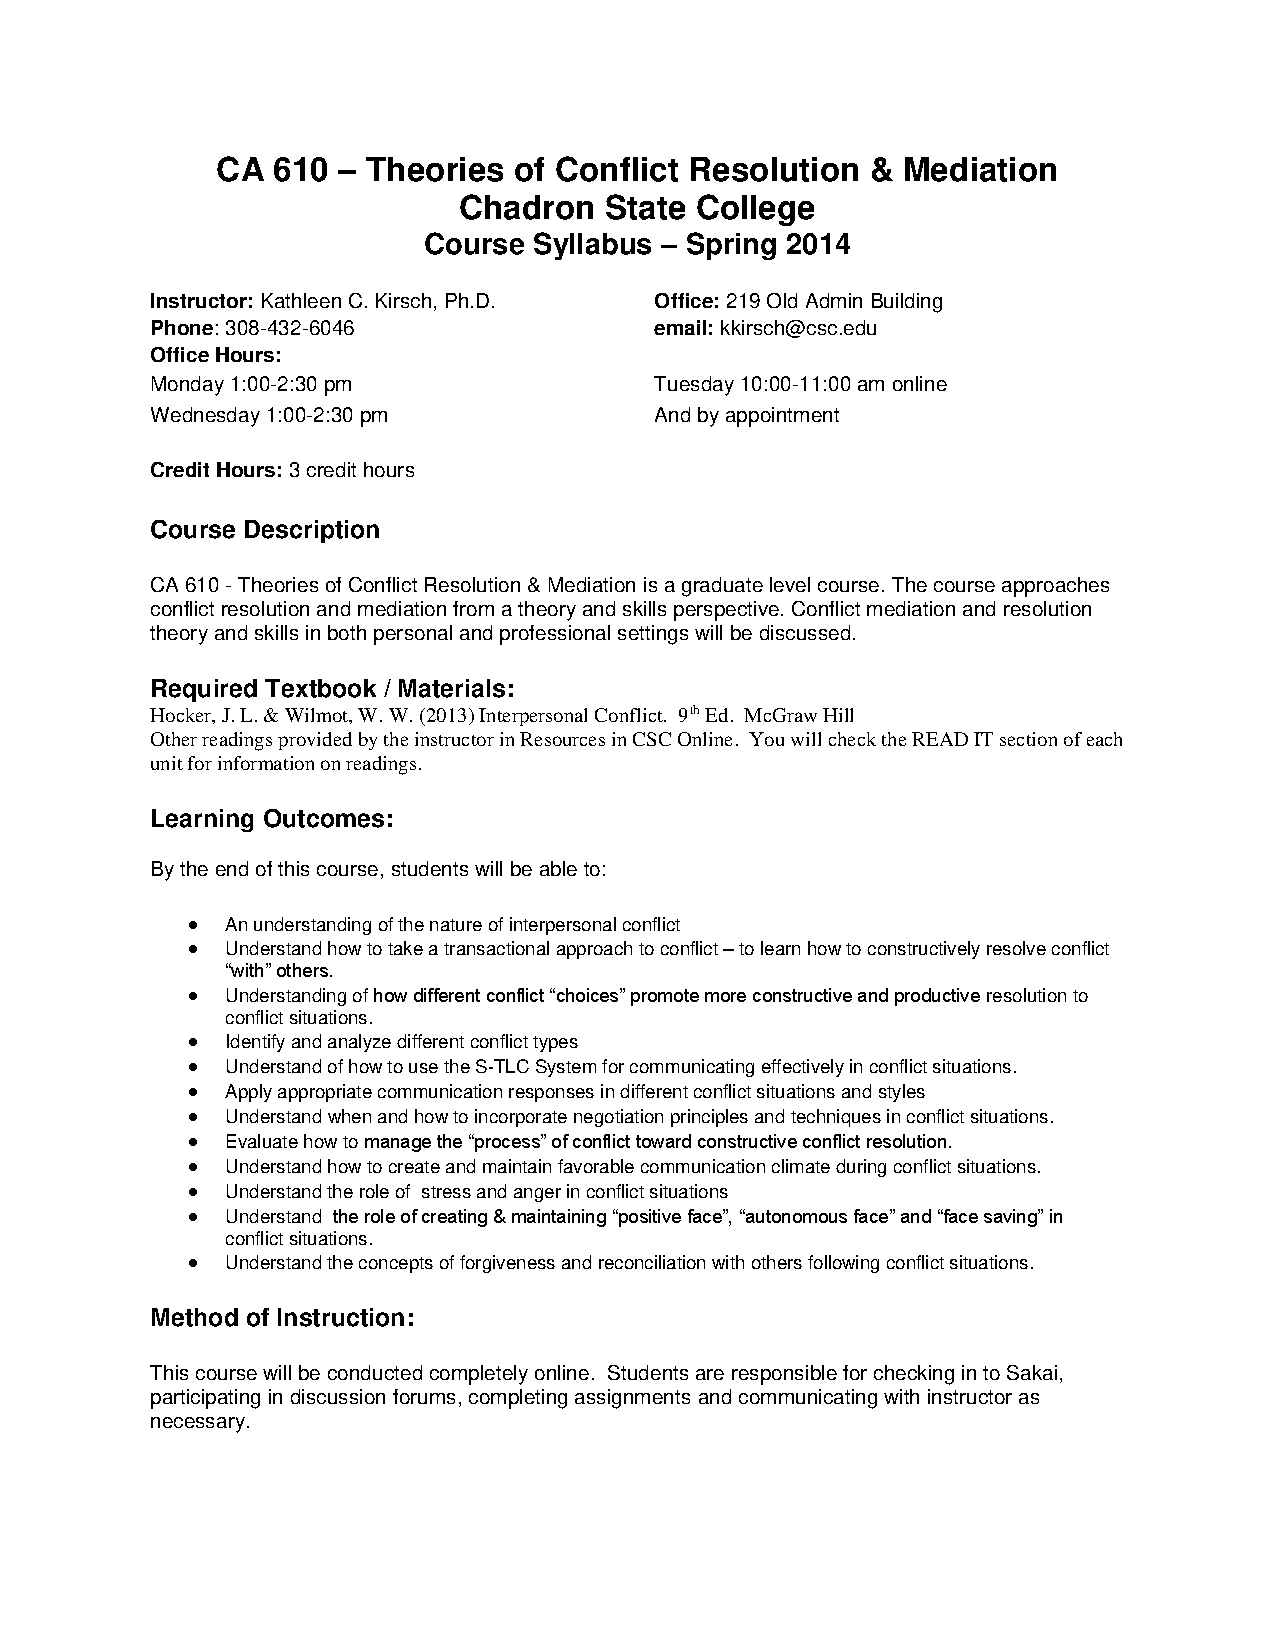
\includepdf[pages=1, pagecommand={\subsubsection{Theories of Conflict Resolution Syllabus}}]{Ca610Spring2014.pdf}
\restoregeometry
\includepdf[pages=2-]{Ca610Spring2014.pdf}
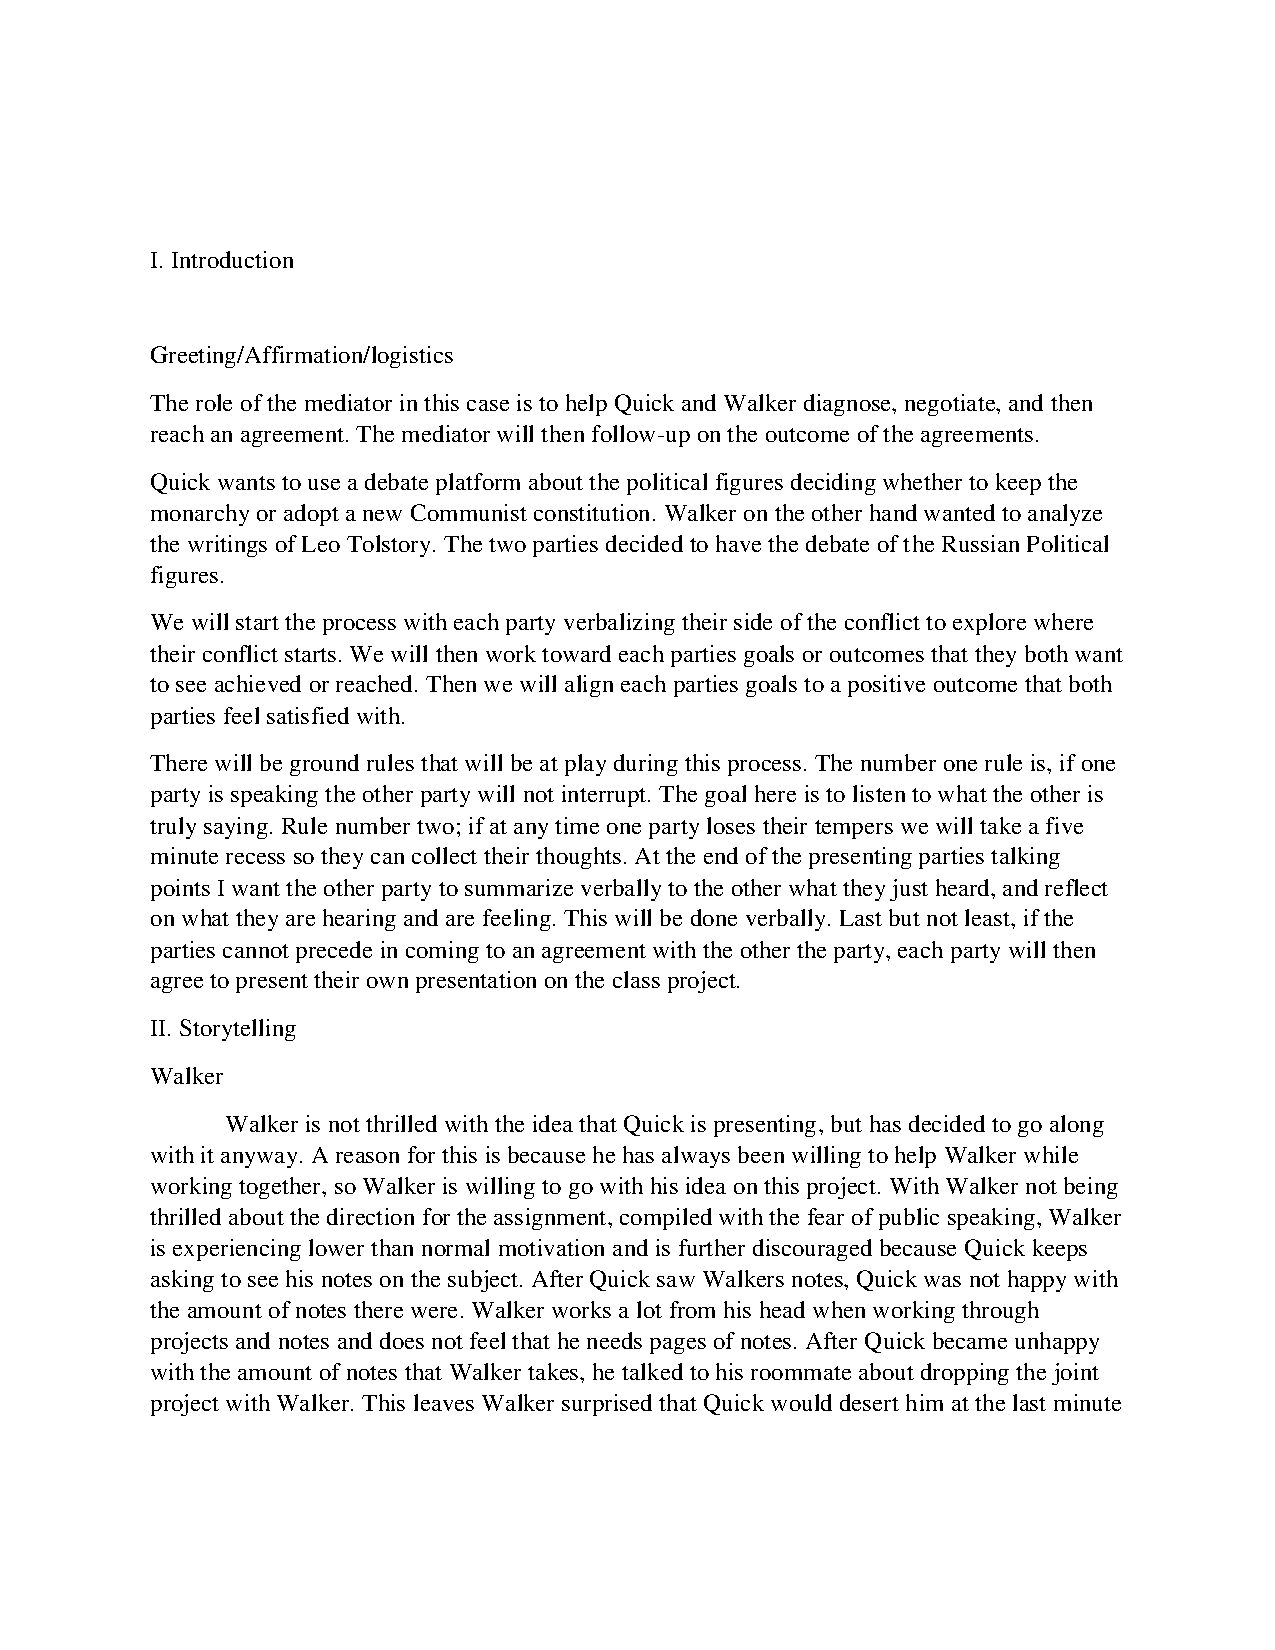
\includepdf[pages=1, pagecommand={\subsubsection{Work Examples}}]{Case_Studies_W-Q.pdf}
\includepdf[pages=2-]{Case_Studies_W-Q.pdf}


% Fall 2014
\subsection{Business Law}
\subsubsection{Reflections}
\paragraph {}
This class should be a required class in any business oriented degree program. I feel that it is so important for everyone to understand legal issues that businesses are presented with everyday. As future leaders we need to stay current with labor regulations environmental regulations and ethical reasoning. Between the text and classroom discussion the class was very interactive with perspectives that ranged from one extreme to the other.
\paragraph {}
I really like the discussions that where included in this class. Dr. Galegos sought out different video or audio clips from different sources such as NPR and various news sites that seemed to be on topic of the readings that week. This was the best way to bridge between traditional classroom teaching and online learning. Every week I looked forward to participating in the discussions because of the relevant material he presented us during the week. On the other side the class assignments were driven to merely provide us with notes for the weekly test. Our assignments were to outline the chapters. For some students this works but does not provide critical thinking needed to fully grasp the many chapters that were assigned weekly. I do understand, however, that the course was a 8 week course with a lot of material that needed to be covered. I just felt that the weekly assignments could have been more meaningful.
\paragraph {}
My undergraduate business law class focused a lot on how to read state statutes, contracts, and how to read court rulings. This class was an extension of that class but focused on regulations nationally and globally. I was not as interested in the chapters which talked about trade regulation and international law as much. This was not because it was poorly described but rather because I have never seen myself in the capacity of international business. The parts of the class I really enjoyed and wanted more of was employee relations and labor management relations and how the regulations work into ethical standards.
\paragraph {}
During and after taking this class I felt that I had grown in relation to how I make organizational decisions. Before these classes thought was not given what legal ramifications exist for each action. The class has really opened my eyes to how we as business leaders need to stay current and possibly develop materials that help other members of the organization to also stay current on regulations and ethical standards as they relate to the type of work we are involved in.
% todo: compile course discussions into one document

\newgeometry{top=.3in}
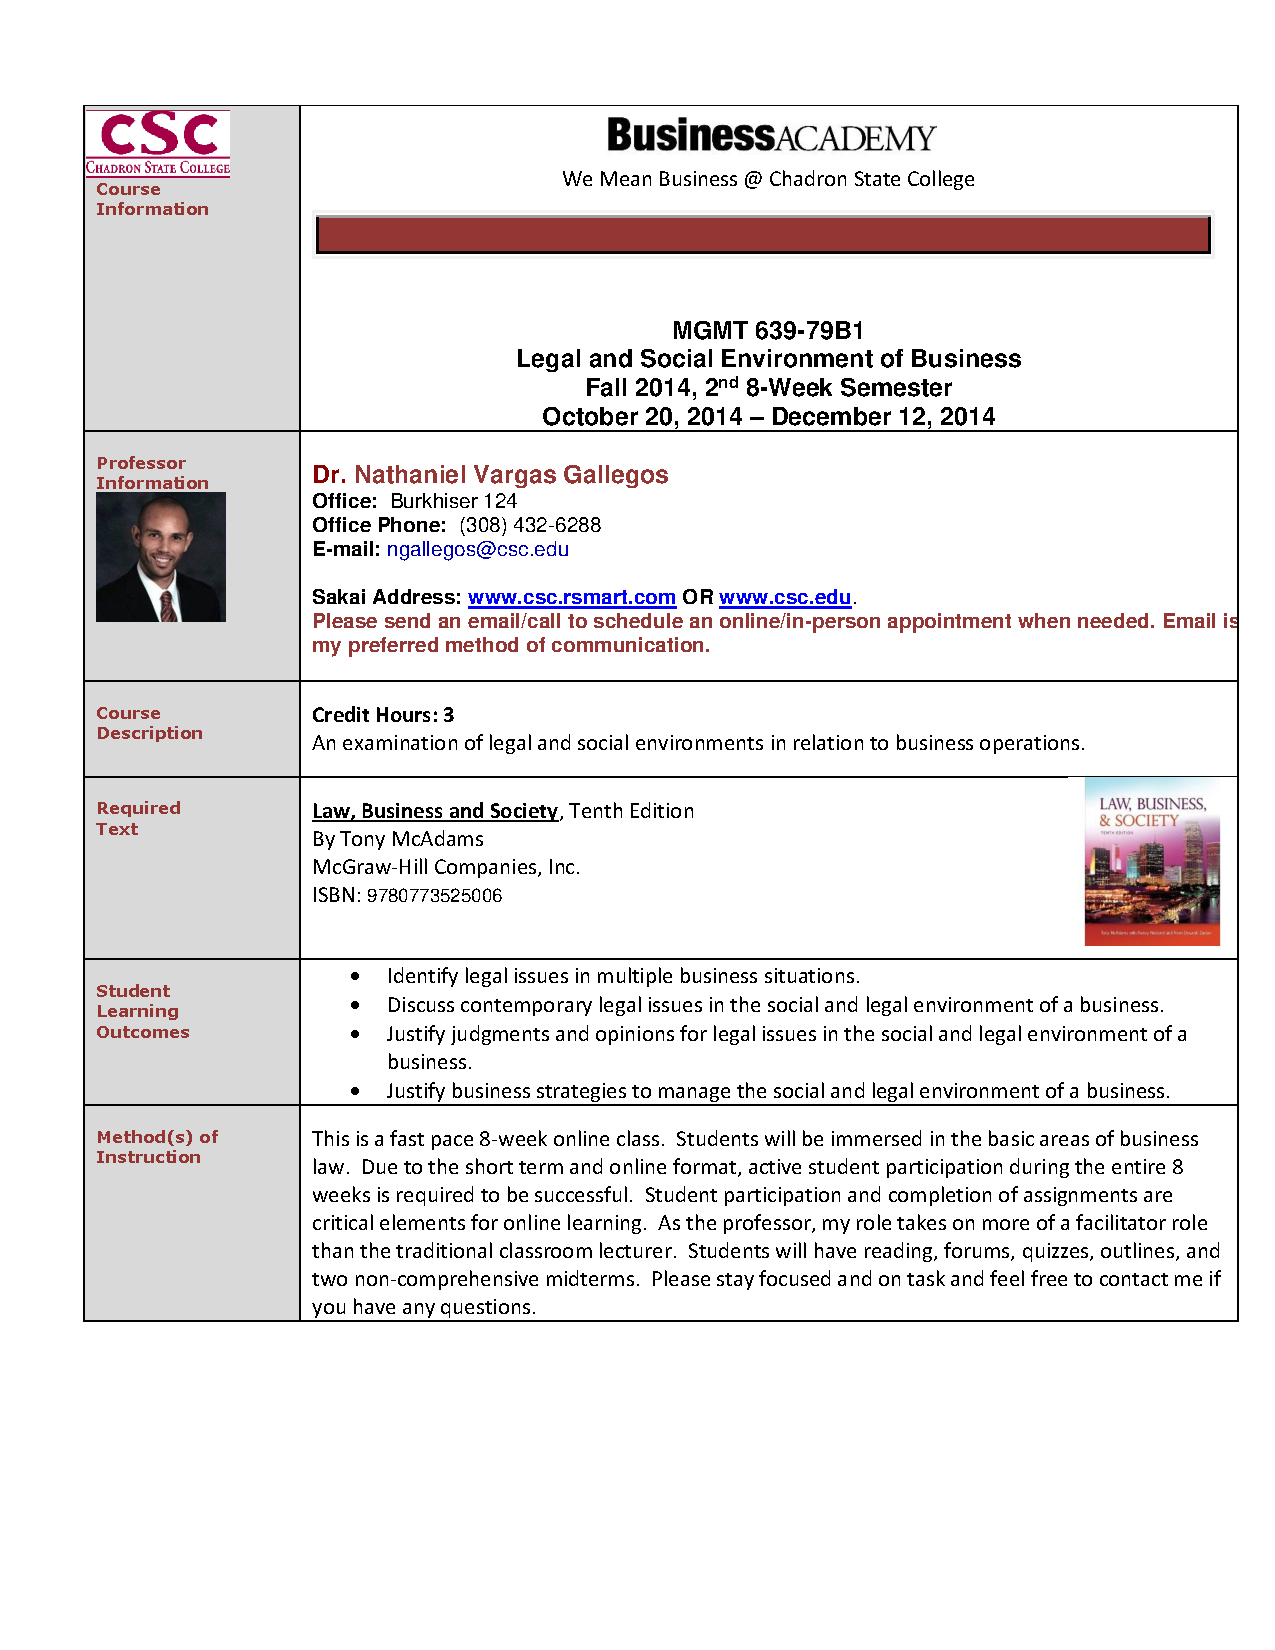
\includepdf[pages=1, pagecommand={\subsection{Business law Syllabus}}]{Syllabus_MGMT639-79B1_NGallegos_1148.pdf}
\restoregeometry
\includepdf[pages=2-]{Syllabus_MGMT639-79B1_NGallegos_1148.pdf}


\subsection{Organizational Behavior}
\subsubsection{Reflections}

\newgeometry{top=.3in}
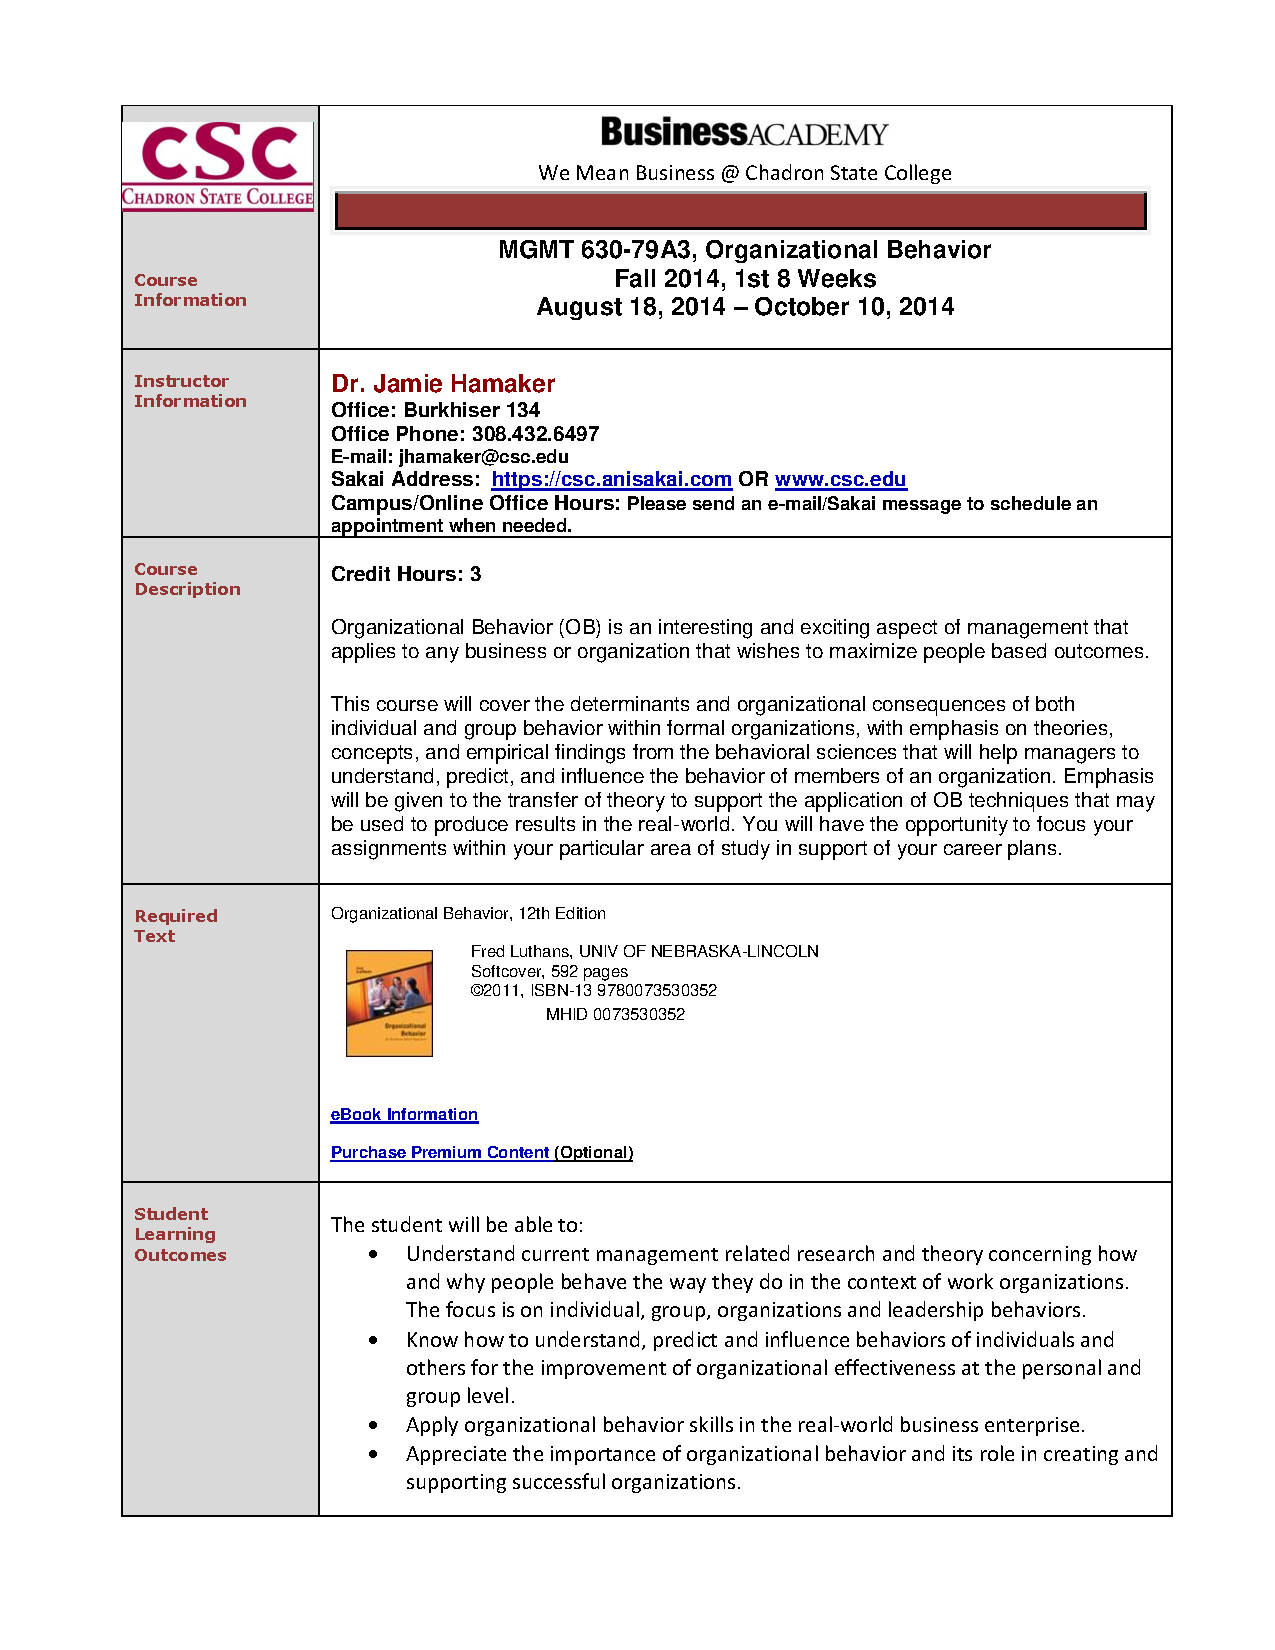
\includepdf[pages=1, pagecommand={\subsubsection{Organizational Behavior Syllabus}}]{Syllabus_MGMT630.pdf}
\restoregeometry
\includepdf[pages=2-]{Syllabus_MGMT630.pdf}
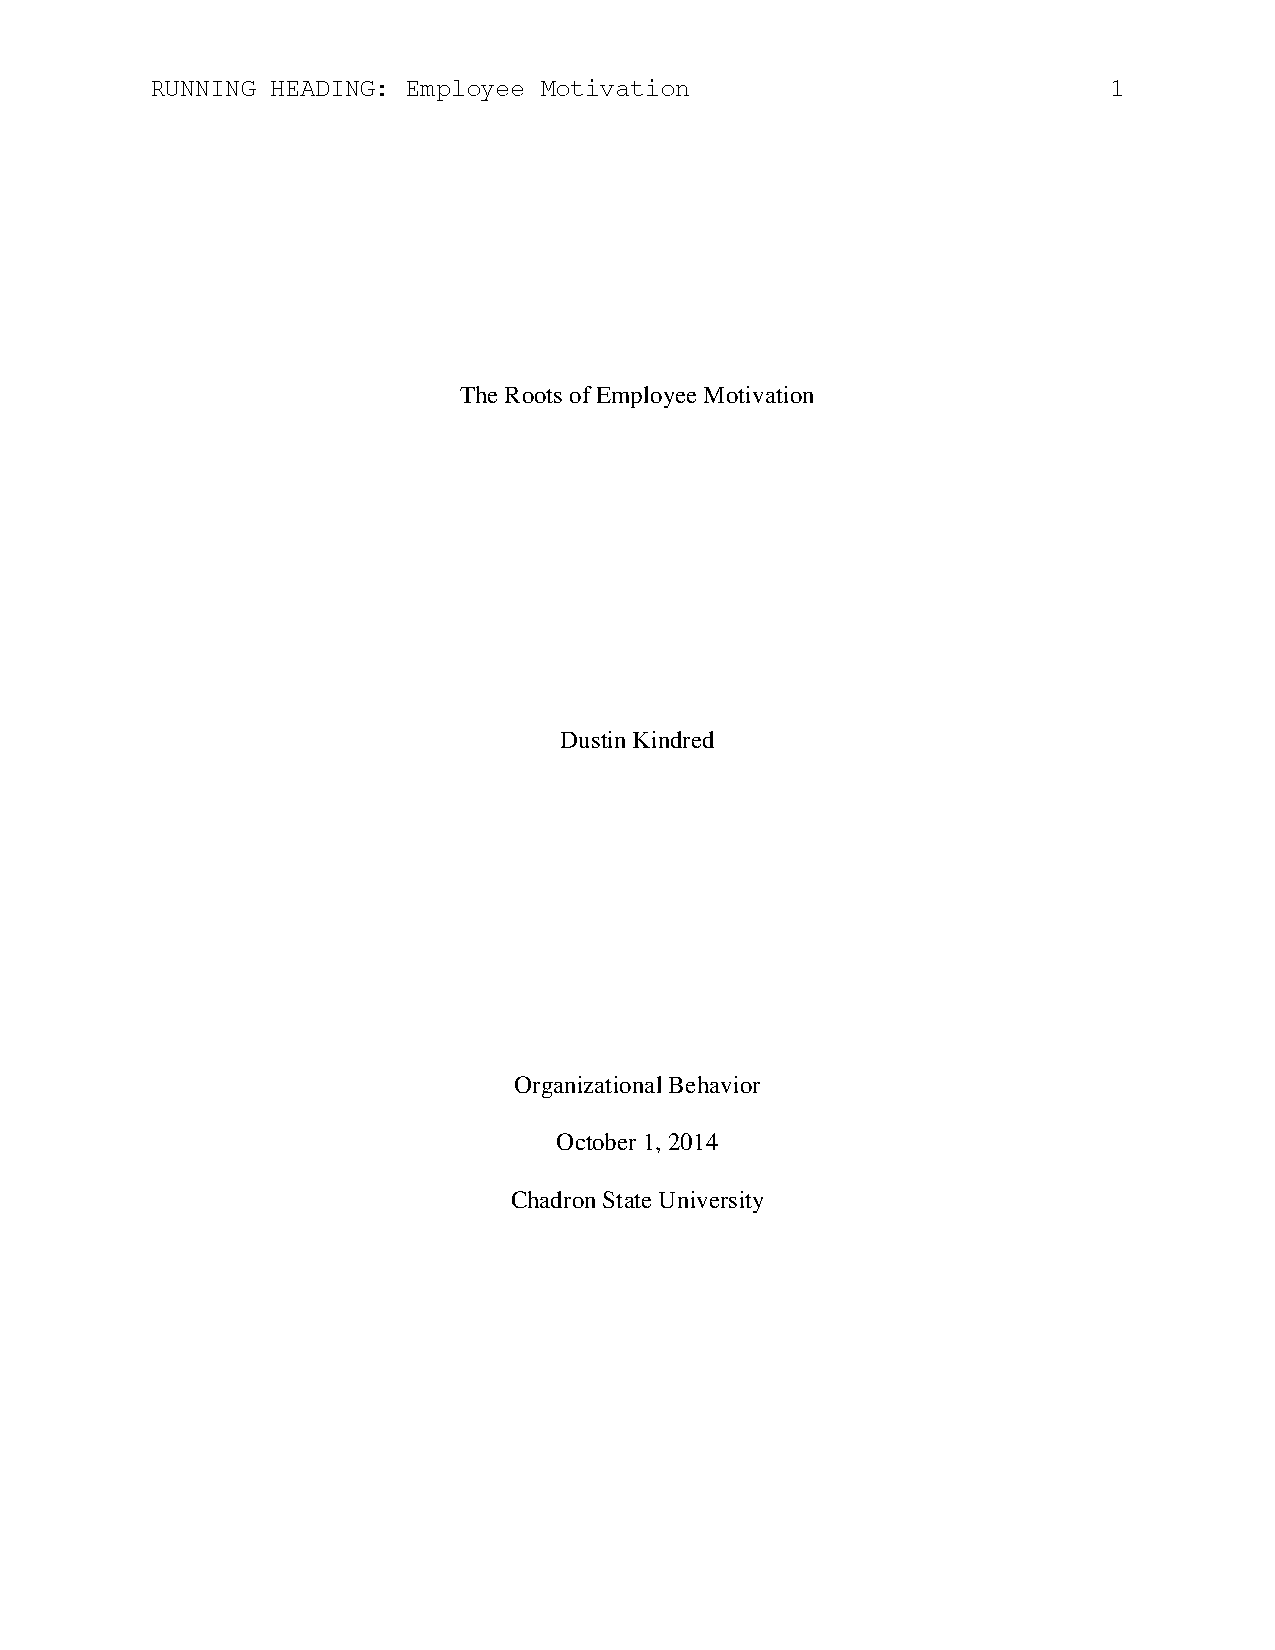
\includepdf[pages=1, pagecommand={\subsubsection{Work Examples}}]{org_behavior_rs.pdf}
\includepdf[pages=2-]{org_behavior_rs.pdf}
% todo: Need  Organizational Behavior Syllabus

% Spring 2015
\subsection{Mathematics for Management}
\subsubsection{Reflections}

\newgeometry{top=.3in}
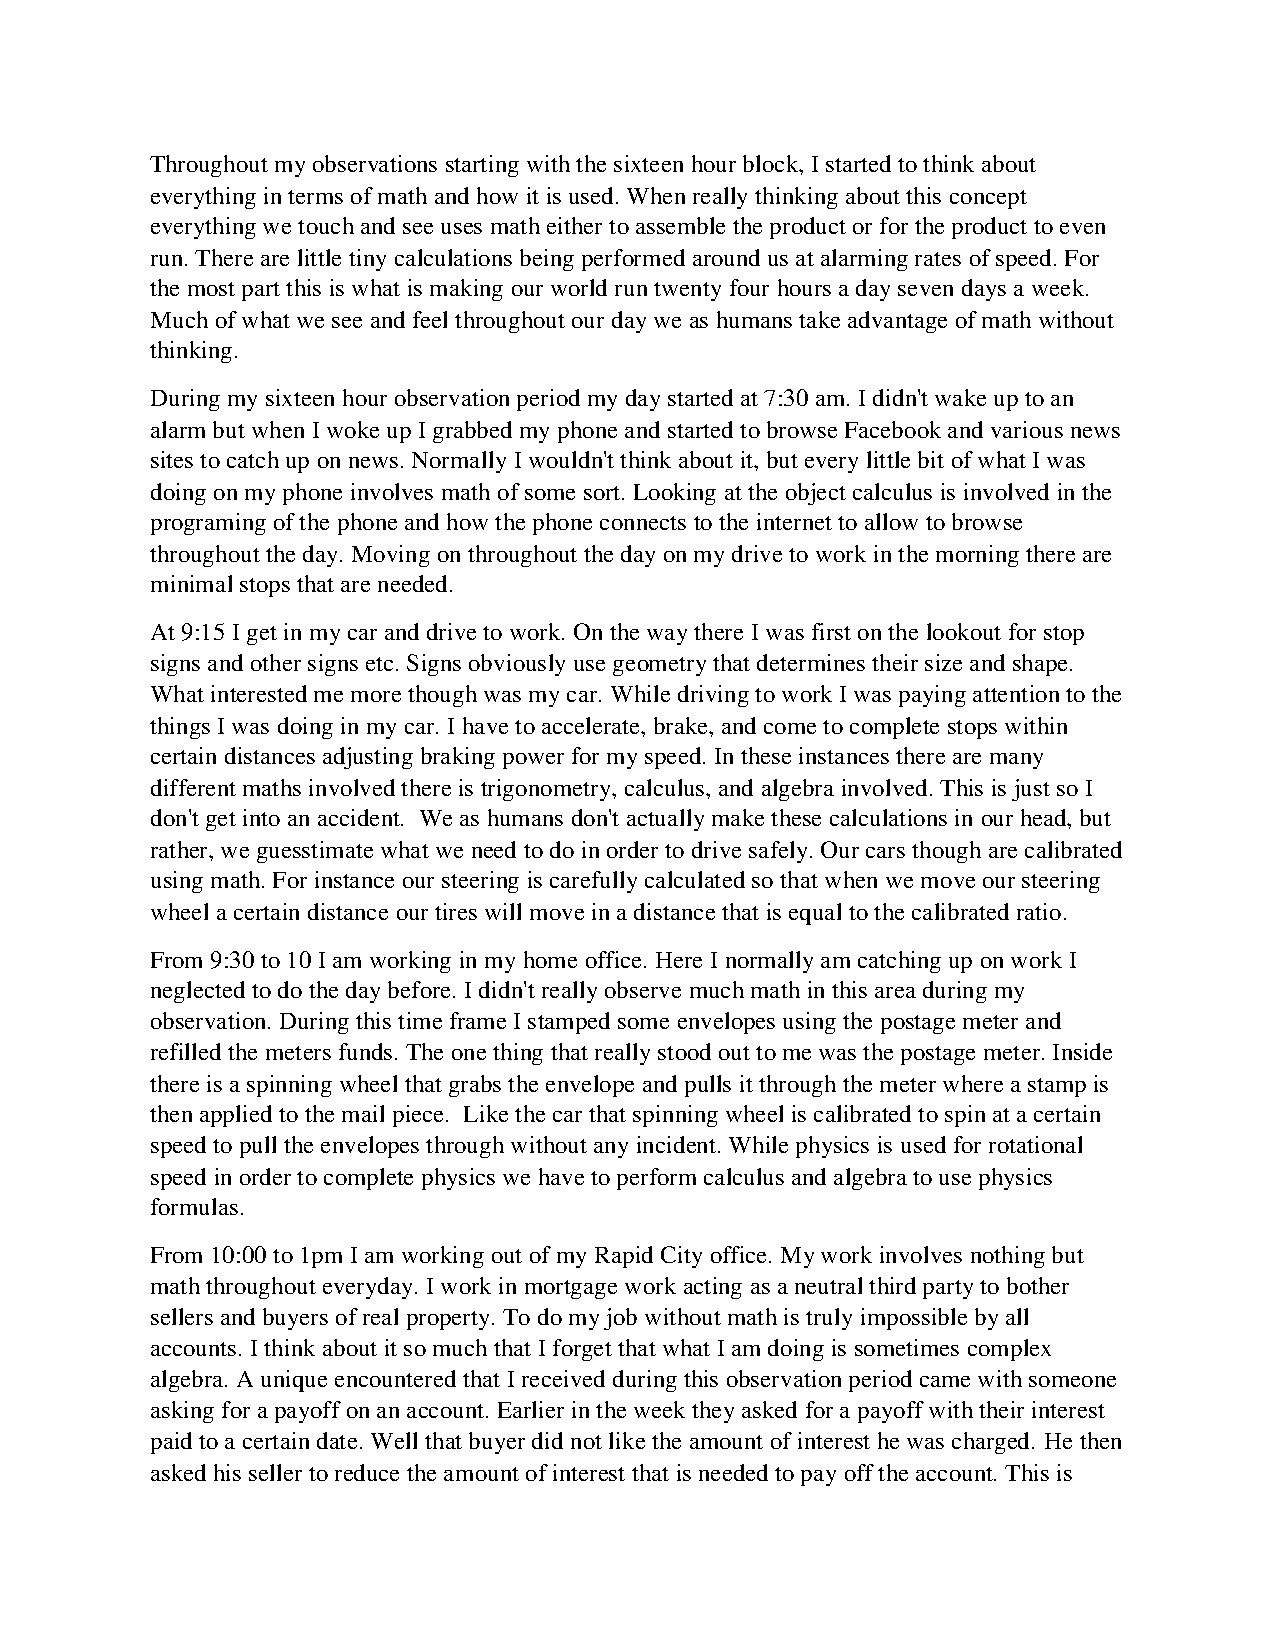
\includepdf[pages=1, pagecommand={\subsubsection{Work Examples}}]{project_4.pdf}
\restoregeometry
\includepdf[pages=2-]{project_4.pdf}
% todo: Need Mathematics for Management Syllabus

\subsection{Public Relations}
\subsubsection{Reflections}

% todo: link Prezi work in document
% todo: Need Syllabus and Work

% Fall 2015
\subsection{Human Capital Management}
\subsubsection{Reflections}

\newgeometry{top=.3in}

\includepdf[pages=1, pagecommand={\subsubsection{Work Examples}}]{hcp_rp.pdf}
\restoregeometry

\includepdf[pages=2-]{hcp_rp.pdf}
% todo: Need Syllabus

\subsection{Marketing Management}
\subsubsection{Reflections}
% todo: Need Syllabus and Work

% Spring 2016
\subsection{Business Internship}



% Part 3
\section{Part III}{Summary and Conclusion}

\bibliographystyle{abbrv}
\bibliography{simple}

\end{document}
This is never printed
